\subsubsection{SITRA}

Øvelsen SITRA gikk ut på at gruppemedlemmene leste to personlige refleksjoner av en situasjon som kunne ha oppstått.
Medlemmene skulle først individuelt kategorisere setningene som situasjon, refleksjon, aksjon eller teori i de to tekstene.
Så skulle disse tolkningene sammenlignes felles i gruppa.
Til å begynne med var det store ulikheter i oppfatningene om hvilke av disse kategoriene som gjaldt for hver setning.
Etter diskusjoner ble det imidlertid enighet om hvor skillet mellom de ulike kategoriene skulle være.

\begin{center}
	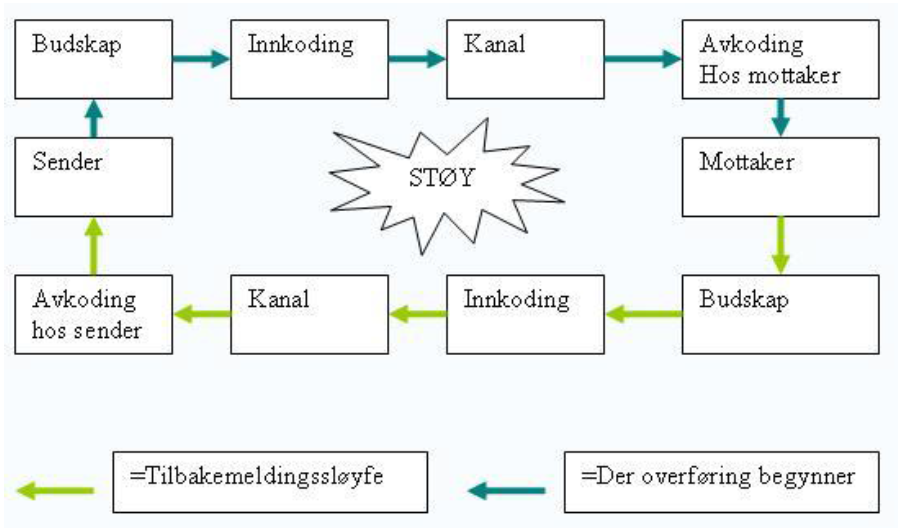
\includegraphics[width=0.5\textwidth]{Kommunikasjon.PNG}
\end{center}

Denne øvelsen trente gruppedeltakerne på kommunikasjon og da spesielt i problemene som oppstår ved semantisk støy.
Semantisk støy handler om hvordan ord og uttrykk blir tolket.
Hvis sender og mottaker operer med ulike referanserammer så kan budskapet bli tolket på en annen måte enn det var tiltenkt eller det kan bli fullstendig uforståelig \cite{prosjekteringsledelse}.
Formålet med SITRA-øvelsen var å bevisstgjøre gruppa på disse referanserammene.